\documentclass[11pt,a4paper]{article}
\usepackage[spanish,provide=*]{babel}
\usepackage{amsmath,amssymb}
\usepackage{geometry}
\geometry{margin=2.3cm,headsep=14pt}
\usepackage{fontspec}
\usepackage{microtype}
\usepackage{pifont}
\usepackage{xcolor}
\usepackage{graphicx}
\usepackage{booktabs}
\usepackage{colortbl}
\usepackage{array}
\usepackage{longtable}
\usepackage{enumitem}
\usepackage[most]{tcolorbox}
\usepackage{fancyhdr}
\usepackage{titlesec}
\usepackage{caption}
\usepackage{etoolbox}
\usepackage{tikz}
\usepackage{hyperref}

% ---- Tokens «Agua viva» (espejo de src/styles/tokens.css, tema claro) ----
\definecolor{agua}{HTML}{EEF7F7}      % --bg
\definecolor{agua2}{HTML}{E9F3F9}     % --bg2
\definecolor{ink}{HTML}{0F2E3D}       % --text
\definecolor{muted}{HTML}{5B7A89}     % --muted
\definecolor{primary}{HTML}{0E7490}   % --primary
\definecolor{accent}{HTML}{0D9488}    % --accent
\definecolor{line}{HTML}{D7E5EA}      % --line
% semáforo de categorías (solo calidad del agua) + tintas AA
\definecolor{catexcelente}{HTML}{0F766E}
\definecolor{catbuena}{HTML}{22C55E}   \definecolor{catbuenaink}{HTML}{052E16}
\definecolor{catregular}{HTML}{EAB308} \definecolor{catregularink}{HTML}{1F2937}
\definecolor{catmarginal}{HTML}{F97316}\definecolor{catmarginalink}{HTML}{431407}
\definecolor{catmala}{HTML}{DC2626}
% semánticos de validación
\definecolor{okink}{HTML}{15803D}
\definecolor{warnink}{HTML}{92600A}

% ---- Tipografía: la Inter real de la app (instancias en fonts/) ----
\setmainfont{Inter}[
  Path=fonts/,
  UprightFont=Inter-Regular.ttf,
  ItalicFont=Inter-Regular.ttf,
  BoldFont=Inter-Bold.ttf,
  BoldItalicFont=Inter-Bold.ttf,
  ItalicFeatures={FakeSlant=0.22},
  BoldItalicFeatures={FakeSlant=0.22},
  FontFace={sb}{n}{Inter-SemiBold.ttf},
  FontFace={sb}{it}{Inter-SemiBold.ttf},
  FontFace={eb}{n}{Inter-ExtraBold.ttf},
  FontFace={eb}{it}{Inter-ExtraBold.ttf},
  Color=ink]
\DeclareRobustCommand{\sbseries}{\fontseries{sb}\selectfont}
\DeclareTextFontCommand{\textsb}{\sbseries}
\DeclareRobustCommand{\ebseries}{\fontseries{eb}\selectfont}
\DeclareTextFontCommand{\texteb}{\ebseries}
% números tabulares en tablas (equivalente a 'tnum' en la web)
\AtBeginEnvironment{tabular}{\addfontfeature{Numbers=Tabular}}
\AtBeginEnvironment{longtable}{\addfontfeature{Numbers=Tabular}}

\hypersetup{colorlinks=true,linkcolor=primary,urlcolor=accent,citecolor=primary,
  pdftitle={Guia de referencia ICA - Indice de Calidad del Agua},pdfauthor={ICA}}
\DeclareCaptionFont{icasb}{\sbseries}
\captionsetup{font=small,labelfont={icasb,color=primary}}
\setlength{\parskip}{0.35em}
\setlength{\parindent}{0pt}
\arrayrulecolor{line}
% último recurso de justificación: evita overfull en líneas con tokens largos inseparables
% (p. ej. «NOM-001-SEMARNAT-2021» en Referencias); no altera el texto, solo el espaciado
\setlength{\emergencystretch}{1.5em}

% ---- Títulos ----
\titleformat{\section}{\color{primary}\Large\ebseries}{\thesection}{0.6em}{}[{\color{line}\titlerule[1pt]}]
\titleformat{\subsection}{\color{accent}\large\sbseries}{\thesubsection}{0.6em}{}
\titleformat{\subsubsection}{\color{muted}\normalsize\sbseries}{\thesubsubsection}{0.6em}{}

% Páginas de Parte: hoja suelta con fondo agua (gradiente como la web)
\titleclass{\part}{page}
\assignpagestyle{\part}{empty}
\titleformat{\part}[display]
  {\centering}
  {\begin{tikzpicture}[remember picture,overlay]
     \shade[top color=agua,bottom color=agua2,shading angle=160]
       (current page.south west) rectangle (current page.north east);
   \end{tikzpicture}%
   \vspace*{3.5cm}
   {\color{muted}\large\sbseries PARTE}\\[6pt]
   {\color{primary}\fontsize{84}{84}\selectfont\ebseries \thepart}}
  {18pt}
  {\color{ink}\fontsize{30}{37}\selectfont\ebseries}
  [{\vspace{10pt}{\color{accent}\rule{0.32\textwidth}{2.5pt}}}]

% ---- Cabeceras y pies ----
\newcommand{\icapill}{\tikz[baseline=(n.base)]\node[fill=primary,text=white,rounded corners=3.2pt,inner xsep=4pt,inner ysep=1.6pt,font=\scriptsize\ebseries](n){ICA};}
\pagestyle{fancy}\fancyhf{}
\lhead{\small\color{muted}\icapill~Índice de Calidad del Agua}
\rhead{\small\color{muted}\leftmark}
\lfoot{\small\color{muted}ica.endho.mx}
\rfoot{\small\color{muted}\thepage}
\renewcommand{\headrulewidth}{0.4pt}
\renewcommand{\footrulewidth}{0.4pt}
\renewcommand{\headrule}{{\color{line}\hrule width\headwidth height\headrulewidth depth 0pt}}
\renewcommand{\footrule}{{\color{line}\hrule width\headwidth height\footrulewidth depth 0pt}}
\renewcommand{\sectionmark}[1]{\markboth{#1}{}}

% ---- Banners (antes «cajas»): fondo translúcido + título saturado, sin marco ----
% Mismos nombres de entorno -> el cuerpo no cambia.
\newtcolorbox{keybox}[1][]{enhanced,breakable,colback=primary!8,colframe=primary!8,
  boxrule=0pt,arc=6pt,left=8pt,right=8pt,top=6pt,bottom=7pt,
  coltitle=primary,fonttitle=\sbseries,colbacktitle=primary!8,
  title={#1},attach title to upper={\par\smallskip}}
\newtcolorbox{warnbox}[1][]{enhanced,breakable,colback=catregular!16,colframe=catregular!16,
  boxrule=0pt,arc=6pt,left=8pt,right=8pt,top=6pt,bottom=7pt,
  coltitle=warnink,fonttitle=\sbseries,colbacktitle=catregular!16,
  title={#1},attach title to upper={\par\smallskip}}
\newtcolorbox{okbox}[1][]{enhanced,breakable,colback=catbuena!13,colframe=catbuena!13,
  boxrule=0pt,arc=6pt,left=8pt,right=8pt,top=6pt,bottom=7pt,
  coltitle=okink,fonttitle=\sbseries,colbacktitle=catbuena!13,
  title={#1},attach title to upper={\par\smallskip}}
\newtcolorbox{sitebox}[1][]{enhanced,breakable,colback=accent!10,colframe=accent!10,
  boxrule=0pt,arc=6pt,left=8pt,right=8pt,top=6pt,bottom=7pt,
  coltitle=accent!70!black,fonttitle=\sbseries,colbacktitle=accent!10,
  title={#1},attach title to upper={\par\smallskip}}

% Ecuaciones: tarjeta blanca con borde --line (como las «tarjetas de código» de Ayuda)
\newcommand{\eqbox}[1]{\begin{tcolorbox}[enhanced,colback=white,colframe=line,boxrule=0.8pt,arc=6pt,
  left=8pt,right=8pt,top=4pt,bottom=4pt]#1\end{tcolorbox}}

% Capturas: tarjeta flotante (borde --line + sombra suave, como .card de la web)
\newcommand{\shot}[2]{\begin{center}\begin{tcolorbox}[enhanced,width=#2,colback=white,colframe=line,
  boxrule=0.6pt,arc=8pt,left=3pt,right=3pt,top=3pt,bottom=2pt,
  drop fuzzy shadow=muted!45]
  \centering\includegraphics[width=\linewidth]{#1}\end{tcolorbox}\end{center}}

% Chip de categoría: pastilla redonda con tinta AA (como .chip-cat de la web)
% \catchip[tinta]{fondo}{texto}   (tinta por defecto: blanca)
\newcommand{\catchip}[3][white]{\tikz[baseline=(n.base)]\node[fill=#2,text=#1,
  rounded corners=8pt,inner xsep=6.5pt,inner ysep=2.6pt,font=\footnotesize\sbseries](n){#3};}

\begin{document}

% =================== PORTADA ===================
\begin{titlepage}
\thispagestyle{empty}
\begin{tikzpicture}[remember picture,overlay]
  \shade[top color=agua,bottom color=agua2,shading angle=160]
    (current page.south west) rectangle (current page.north east);
\end{tikzpicture}%

\vspace*{1.8cm}
{\noindent\tikz[baseline=(n.base)]\node[left color=primary,right color=accent,text=white,
  rounded corners=7pt,inner xsep=11pt,inner ysep=6.5pt,font=\LARGE\ebseries](n){ICA};\par}

\vspace{1.5cm}
{\noindent\fontsize{38}{45}\selectfont\ebseries Índice de Calidad del Agua\par}
\vspace{10pt}
{\noindent\LARGE\color{primary}\sbseries Guía de referencia y manual de usuario\par}

\vspace{1.6cm}
\begin{tcolorbox}[enhanced,width=\textwidth,colback=white,colframe=white,boxrule=0pt,
  arc=10pt,left=16pt,right=16pt,top=13pt,bottom=13pt,drop fuzzy shadow=muted!45]
\large
Una aplicación web para calcular el \textbf{CCME Water Quality Index} directamente en el
navegador, orientada a aguas mexicanas y desarrollada como respuesta a la solicitud de un
\textbf{Índice de Calidad del Agua} para SEMARNAT.

\vspace{0.7em}
{\normalsize\color{muted}
Este documento reúne, en un solo lugar: el fundamento y las ecuaciones del índice; la
documentación completa del archivo de \emph{guías} (Guidelines) con sus tipos de regla y fórmulas;
un ejemplo validado de extremo a extremo; y una guía de uso del sitio \textbf{ica.endho.mx}.}
\end{tcolorbox}

\vfill
\begin{tcolorbox}[colback=white!55,colframe=white!55,arc=6pt,left=10pt,right=10pt,top=7pt,bottom=7pt]
\small
\textbf{Sitio:} \href{https://ica.endho.mx}{ica.endho.mx} \quad\textbullet\quad
\textbf{Código:} github.com/oscolv/ica \quad\textbullet\quad
\textbf{Privacidad:} todo el cálculo ocurre en tu navegador; ningún dato se sube a un servidor.
\end{tcolorbox}
{\small\color{muted}Documento de referencia técnica · \today}
\end{titlepage}

\tableofcontents
\newpage

% =================== PARTE I ===================
\part{El índice}

\section{Qué es ICA}
\textbf{ICA} es una aplicación web que calcula el \textbf{CCME Water Quality Index (CCME WQI)} y comunica
el resultado de forma clara. Convierte una montaña de datos de monitoreo —muchos parámetros, muchas
fechas, varias estaciones— en un único número entre \textbf{0} (peor) y \textbf{100} (mejor) y una
categoría verbal, con narrativa automática y gráficas.

\begin{sitebox}[La herramienta, en una frase]
ICA responde ``¿qué tan lejos está esta agua de cumplir sus propias reglas?'' midiendo la falla en
tres dimensiones —cuántos parámetros, con qué frecuencia y por cuánto— y combinándolas
geométricamente para que ningún problema grave se diluya. Todo sucede en tu navegador.
\end{sitebox}

El índice fue endosado por el Canadian Council of Ministers of the Environment (CCME) en 2001 y
actualizado en 2017; deriva del índice de British Columbia (Rocchini y Swain, 1995) con
modificaciones de Alberta. ICA lo lleva al navegador, en español, con presets y una plantilla
pensada para México.

\subsection{Qué es y qué no es el CCME WQI}
\begin{keybox}[La idea central]
El índice \textbf{no compara concentraciones entre sí} (no tendría sentido comparar µg/L de un
pesticida contra mg/L de un ión mayor). Cada medición se compara \textbf{únicamente contra su propia
guía}. La pregunta para cada dato no es ``¿cuánto hay?'' sino ``¿cumple su límite, y por cuánto se
pasa?''. Así todo se traduce a una moneda común: \textbf{distancia respecto a lo aceptable}.
\end{keybox}

\begin{minipage}[t]{0.48\textwidth}
\textbf{Qué es}
\begin{itemize}[leftmargin=1.1em,nosep]
  \item Una herramienta de \textbf{comunicación}.
  \item Un marco \textbf{relativo a guías} definidas por el usuario.
  \item \textbf{Flexible}: parámetros, guías, periodo y cuerpo de agua.
  \item \textbf{Sin ponderaciones arbitrarias}: la toxicidad vive en la guía.
\end{itemize}
\end{minipage}\hfill
\begin{minipage}[t]{0.48\textwidth}
\textbf{Qué NO es}
\begin{itemize}[leftmargin=1.1em,nosep]
  \item Un \textbf{diagnóstico}: dice que el agua está mal, no por qué.
  \item \textbf{Absoluto}: cambia si cambian parámetros o guías.
  \item Un captador de \textbf{eventos transitorios} (derrames).
  \item Un \textbf{sustituto} de una evaluación detallada.
\end{itemize}
\end{minipage}

\section{Los tres factores}
``Mala calidad'' puede significar tres cosas distintas; el índice las captura por separado.

\begin{center}\renewcommand{\arraystretch}{1.3}
\begin{tabular}{@{}p{2.3cm} p{4.1cm} p{7.6cm}@{}}
\toprule
\textbf{Factor} & \textbf{Pregunta} & \textbf{Interpretación} \\ \midrule
$F_1$ \small Scope & ¿\emph{Cuántos} parámetros fallan al menos una vez? & Extensión del problema. \\
$F_2$ \small Frequency & ¿\emph{Con qué frecuencia} fallan? & Persistencia. \\
$F_3$ \small Amplitude & ¿\emph{Por cuánto} se pasan de la guía? & Severidad. \\ \bottomrule
\end{tabular}
\end{center}

Los tres se tratan como \textbf{ejes perpendiculares} en un espacio tridimensional; el índice es la
longitud de ese vector, normalizada. La elección geométrica es deliberada: hace que \textbf{un solo
factor alto ya arrastre el resultado hacia abajo}, impidiendo que un problema grave se esconda
detrás de parámetros que sí cumplen.

\section{Las ecuaciones, al detalle}
Definidos el cuerpo de agua, el periodo, los parámetros y sus guías, se calculan los tres factores.

\subsection{$F_1$ — Scope (alcance)}
Porcentaje de \emph{parámetros} que no cumplen su guía \textbf{al menos una vez}.
\eqbox{\[F_1=\left(\frac{\text{parámetros fallidos}}{\text{parámetros totales}}\right)\times 100\tag{1}\]}

\subsection{$F_2$ — Frequency (frecuencia)}
Porcentaje de \emph{pruebas individuales} (cada dato de cada parámetro en cada fecha) que no cumplen.
\eqbox{\[F_2=\left(\frac{\text{pruebas fallidas}}{\text{pruebas totales}}\right)\times 100\tag{2}\]}

\subsection{$F_3$ — Amplitude (amplitud), en tres pasos}
\textbf{Paso i — Excursión.} Cuántas veces un valor rebasa su guía:
\eqbox{
Si el valor \textbf{no debe superar} la guía: \(\ \text{excursión}_i=\left(\dfrac{\text{valor}_i}{\text{objetivo}_j}\right)-1\ \) (3a)\\[3pt]
Si el valor \textbf{no debe caer por debajo} (p. ej. oxígeno disuelto): \(\ \text{excursión}_i=\left(\dfrac{\text{objetivo}_j}{\text{valor}_i}\right)-1\ \) (3b)}

\begin{keybox}[El detalle que domina el resultado]
La excursión se mide contra la \textbf{misma guía} que decide si el parámetro falla. Por eso una guía
pequeña produce excursiones enormes: un aluminio de $0.166$ mg/L contra una guía de $0.005$ mg/L da
$0.166/0.005-1=32$. La guía no solo decide \emph{si} falla, también \emph{por cuánto}.
\end{keybox}

\textbf{Paso ii — Suma normalizada de excursiones (nse).} Se dividen entre \emph{todas} las pruebas
(las que cumplen y las que no):
\eqbox{\[nse=\frac{\sum_{i=1}^{n}\text{excursión}_i}{\#\ \text{de pruebas}}\tag{4}\]}

\textbf{Paso iii — Escalado asintótico.} $F_3$ comprime cualquier $nse$ al rango 0–100:
\eqbox{\[F_3=\left(\frac{nse}{0.01\,nse+0.01}\right)\tag{5}\]}

\begin{figure}[h]\centering
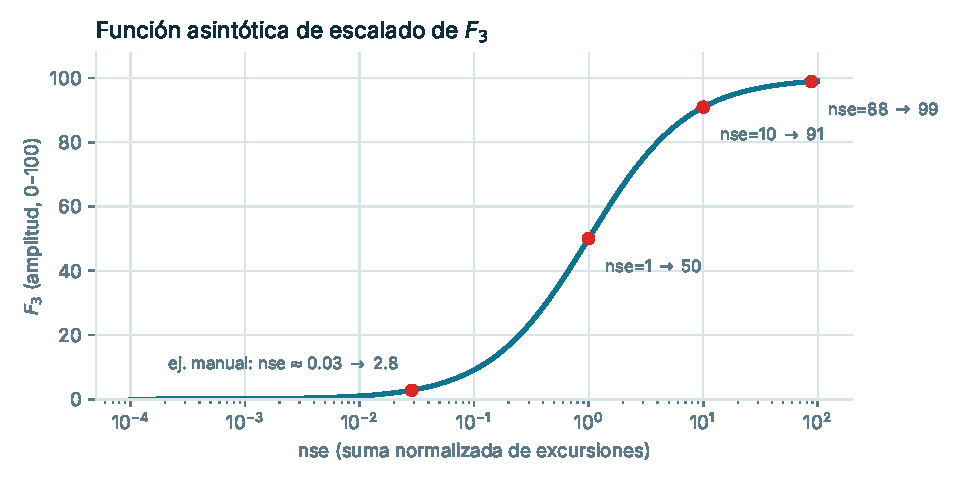
\includegraphics[width=0.74\textwidth]{manual_assets/f3_curve.pdf}
\caption{Función asintótica de $F_3$ (eje horizontal logarítmico). Las constantes $0.01$ son fijas del
manual: pasarse \emph{un poco} castiga mucho; pasarse \emph{muchísimo} ya casi no cambia el resultado
(saturación en 100). Esto atenúa la influencia indebida de parámetros con rango de órdenes de magnitud.}
\end{figure}

\subsection{Índice final — suma vectorial}
\eqbox{\[\text{CCME WQI}=100-\left(\frac{\sqrt{F_1^{\,2}+F_2^{\,2}+F_3^{\,2}}}{1.732}\right)\tag{6}\]}
El divisor $1.732\approx\sqrt{3}$ normaliza a 0–100 (el máximo de la raíz es $\sqrt{3\cdot100^2}=173.2$);
se resta de 100 para que \textbf{más alto = mejor}.

\section{Categorías}
\begin{center}\renewcommand{\arraystretch}{1.7}
\begin{tabular}{@{}l l p{9.2cm}@{}}
\toprule
{\footnotesize\sbseries\color{muted}CATEGORÍA} & {\footnotesize\sbseries\color{muted}RANGO} & {\leavevmode\footnotesize\sbseries\color{muted}SIGNIFICADO} \\ \midrule
\catchip{catexcelente}{Excelente} & 95--100 & Ausencia virtual de amenaza; condiciones casi prístinas. \\
\catchip[catbuenaink]{catbuena}{Buena} & 80--94 & Grado menor de amenaza; rara vez se aparta de lo deseable. \\
\catchip[catregularink]{catregular}{Regular} & 65--79 & Ocasionalmente amenazada; a veces se aparta de lo deseable. \\
\catchip[catmarginalink]{catmarginal}{Marginal} & 45--64 & Frecuentemente amenazada o deteriorada. \\
\catchip{catmala}{Mala} & 0--44 & Casi siempre amenazada o deteriorada. \\ \bottomrule
\end{tabular}
\end{center}
\begin{warnbox}[Cuidado con las fronteras]
Los cortes (95, 80, 65, 45) son juicio experto, no ciencia dura. Un sitio cerca de una frontera puede
cambiar de categoría por una variación mínima; conviene usar juicio profesional.
\end{warnbox}

\section{Preparación de datos: supuestos y matices}
\begin{description}[leftmargin=1.3em,style=nextline]
  \item[No detectados (``$<x$'' o ``L$x$'').] Se usan como observaciones \textbf{en el valor del límite de detección}.
  \item[Límite de detección $>$ guía.] Se usa el LD como guía (evita falsos positivos con excursiones enormes).
  \item[Datos faltantes.] Se excluyen del conteo de pruebas.
  \item[Parámetros sin guía.] No entran en el índice.
\end{description}
\begin{center}\renewcommand{\arraystretch}{1.15}
\begin{tabular}{@{}p{5cm} p{9.6cm}@{}}
\toprule \textbf{Aspecto} & \textbf{Recomendación} \\ \midrule
Número de parámetros & Mínimo absoluto 4; \textbf{recomendado 8 a 20}. \\
Muestras por año & $\sim$10 para ríos; mínimo 4 visitas/año. \\
Periodo & 1 año para reportar mejoras; $\sim$3 años para estado. \\
Comparaciones válidas & Solo con \emph{iguales} parámetros, guías, periodos y número de muestras. \\ \bottomrule
\end{tabular}
\end{center}

% =================== PARTE II ===================
\part{La guía (Guidelines)}

\section{Qué es el archivo de guías}
El archivo \texttt{Guidelines.csv} es la \textbf{tabla de objetivos} contra la cual el índice compara
cada medición. No forma parte del algoritmo (que solo define \emph{cómo} se combinan los
incumplimientos); es la pieza que define \emph{qué} se considera un incumplimiento. Cambiar una guía
cambia el veredicto, por lo que su origen debe documentarse tanto como el cálculo.

\begin{center}\renewcommand{\arraystretch}{1.25}
\begin{longtable}{@{}p{3.6cm} p{11.4cm}@{}}
\toprule \textbf{Columna} & \textbf{Significado} \\ \midrule\endhead
\texttt{PARAMETER\_ID} & Identificador; debe coincidir \textbf{exactamente} con la columna de datos. \\
\texttt{EXCEED\_IF} & Tipo de regla de incumplimiento (el ``motor''). \\
\texttt{LOWER/UPPER\_LIMIT} & Umbrales mínimo / máximo. \\
\texttt{HARDNESS\_LOWER/UPPER} & Rango de dureza (mg/L CaCO$_3$) para escalones. \\
\texttt{SEASON\_START/FINISH} & Ventana de fechas para reglas estacionales. \\
\texttt{GUIDELINE\_SOURCE} & Procedencia y versión (trazabilidad). \\
\texttt{UNIT\_ID} & Unidad del objetivo. \\ \bottomrule
\end{longtable}
\end{center}

\section{Los tipos de regla (\texttt{EXCEED\_IF})}
Cada regla decide (a) si una medición incumple y (b) qué objetivo se usa para la excursión. La
siguiente tabla resume los \textbf{tipos de regla que ICA soporta}, compatibles con el formato de
guías del CCME.

\begin{center}\renewcommand{\arraystretch}{1.35}
\begin{longtable}{@{}p{4.6cm} p{6.6cm} p{3.0cm}@{}}
\toprule \textbf{Código} & \textbf{Qué hace} & \textbf{Necesita} \\ \midrule\endhead
\texttt{>} / \texttt{<} / \texttt{<>} & máximo / mínimo / rango & límite(s) \\
\texttt{Hardness} & escalones por dureza (Plomo) & columna dureza \\
\texttt{Season} & límite por fecha (Fósforo, Turbidez) & ventanas de fecha \\
\texttt{COMPUTE} & \textbf{amoníaco no ionizado} (¡no genérico!) & pH + temperatura \\
\texttt{pHDependCCME} & aluminio por pH & columna pH \\
\texttt{CdHardness}, \texttt{CuHardness}, \texttt{NiHardness}, \texttt{PbHardness}, \texttt{ZnHardness} & fórmulas por dureza (cadmio, cobre, níquel, plomo, zinc) & columna dureza \\ \bottomrule
\end{longtable}
\end{center}

\begin{warnbox}[Nota importante: \texttt{COMPUTE} corresponde al amoníaco]
En este formato, \texttt{COMPUTE} calcula \emph{específicamente} el amoníaco no ionizado (a partir de
pH y temperatura); \textbf{no} es un ``computa la fórmula que corresponda'' genérico. Por eso, para los
metales que dependen de la dureza, usa \texttt{CuHardness}, \texttt{NiHardness}, \texttt{PbHardness}
—no \texttt{COMPUTE}—. Es el error más común al adaptar guías.
\end{warnbox}

\section{Guías dependientes de la química: fundamento y fórmulas}
La toxicidad real no siempre depende solo de la concentración.

\subsection{Por qué la dureza importa}
La dureza (Ca$^{2+}$, Mg$^{2+}$, como mg/L de CaCO$_3$) \textbf{reduce la toxicidad} de muchos metales:
los cationes compiten con el metal por los sitios de unión en las branquias. Por eso, en aguas duras,
la guía puede ser más alta sin aumentar el riesgo real.

\begin{figure}[h]\centering
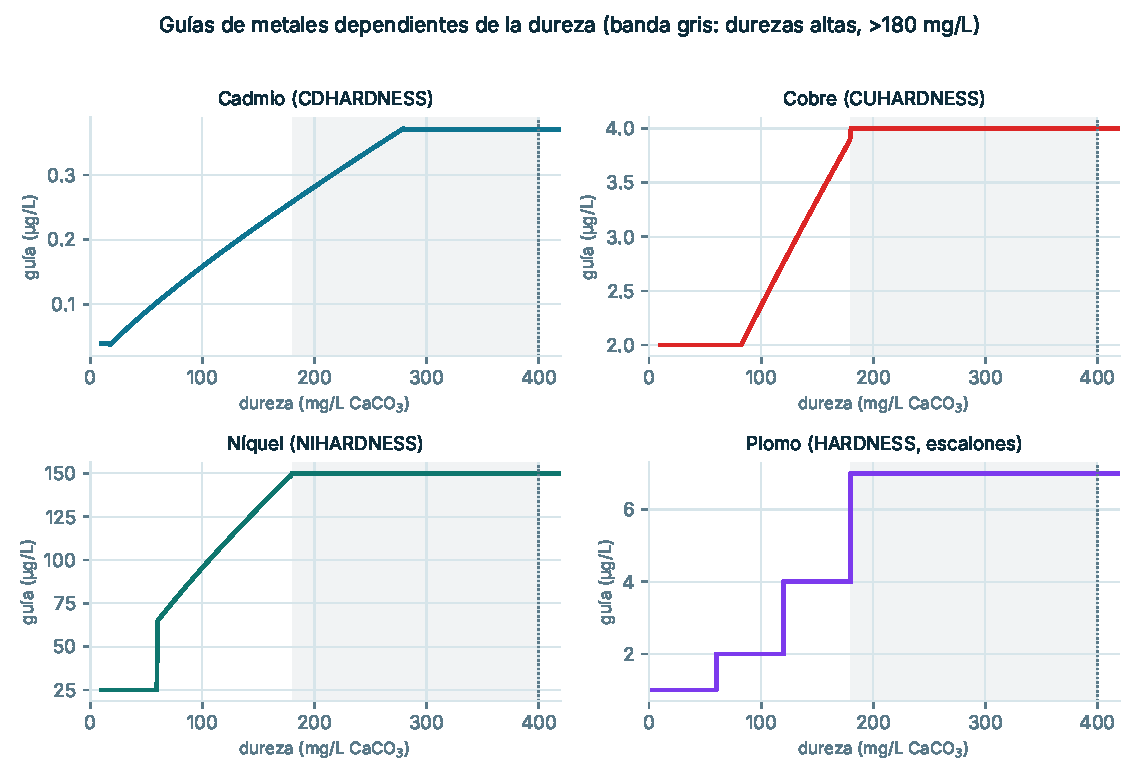
\includegraphics[width=0.92\textwidth]{manual_assets/hardness_guides.pdf}
\caption{Guías de metales en función de la dureza. La banda gris marca durezas altas ($>180$ mg/L),
donde cobre, níquel y plomo alcanzan su techo.}
\end{figure}

\subsection{Las fórmulas (guías CCME dependientes de la química)}
\eqbox{
\textbf{Cadmio:} $H<17\to0.04$; $H>280\to0.37$; si no $10^{\,0.83\log_{10}H-2.46}$ µg/L\\[2pt]
\textbf{Cobre:} $H<82\to2$; $H>180\to4$; si no $0.2\,e^{\,0.8545\ln H-1.465}$ µg/L\\[2pt]
\textbf{Níquel:} $H\le60\to25$; $H>180\to150$; si no $e^{\,0.76\ln H+1.06}$ µg/L\\[2pt]
\textbf{Plomo:} $H<60\to1$; $H>180\to7$; si no $e^{\,1.273\ln H-4.705}$ µg/L\\[2pt]
\textbf{Zinc:} $H<90\to7.5$; si no $7.5+0.75(H-90)$ µg/L\\[2pt]
\textbf{Aluminio (pH):} $pH<6.5\to0.005$; si no $0.1$ mg/L\\[2pt]
\textbf{Amoníaco (fracción no ionizada):} $f=1/\!\left(1+10^{\,0.09018+2729.92/(273.2+T)-pH}\right)$
}

\section{Cómo se eligen los valores}
Todos los valores CCME provienen de las \emph{Canadian Water Quality Guidelines for the Protection of
Aquatic Life}. El procedimiento general: reunir estudios de toxicidad de calidad; identificar el efecto
sobre la \textbf{especie más sensible}; aplicar un \textbf{factor de seguridad}; distinguir exposición
crónica (la usada con muestreo mensual) de aguda; y, cuando la biodisponibilidad depende de la química,
expresar la guía como \textbf{función} de dureza o pH.

\section{Catálogo de parámetros CCME (completo)}
El preset \textbf{CCME — vida acuática} de ICA trae el conjunto oficial completo. La tabla lista todos
los parámetros con su guía, unidad, tipo de regla y versión de la fuente. Léela menos como una lista
para memorizar y más como un \textbf{modelo}: observa cómo el \emph{tipo de regla} y la \emph{magnitud
del valor} cambian según la naturaleza de cada parámetro.

\begin{center}\footnotesize\renewcommand{\arraystretch}{1.22}
\begin{longtable}{@{}p{4.0cm} p{3.0cm} p{1.7cm} p{2.5cm} p{2.2cm}@{}}
\toprule \textbf{Parámetro} & \textbf{Guía} & \textbf{Unidad} & \textbf{Regla} & \textbf{Fuente} \\ \midrule\endhead
Aluminio total & 0.005 / 0.1 (según pH) & mg/L & pH & CCME 1987 \\
Amoníaco no ionizado & 0.0152 & mg/L (N) & $>$ & CCME 2001 \\
Amoníaco total & computa (pH, temp) & mg/L (N) & COMPUTE & CCME 2001 \\
Arsénico total & 5 & µg/L & $>$ & CCME 1997 \\
Cadmio total & fórmula (dureza) & µg/L & dureza & CCME 1996 \\
Cloruro & 120 & mg/L & $>$ & CCME 2011 \\
Cobre total & 2 / fórmula / 4 & µg/L & dureza & CCME 1987 \\
Cromo (III) & 8.9 & µg/L & $>$ & CCME 1997 \\
Cromo (VI) & 1 & µg/L & $>$ & CCME 1997 \\
Fósforo total & 0.03 / 0.02 / 0.03 & mg/L & estación & CCME 2004 \\
Hierro total & 0.3 & mg/L & $>$ & CCME 1987 \\
Mercurio inorgánico & 0.026 & µg/L & $>$ & CCME 2003 \\
Metilmercurio & 0.004 & µg/L & $>$ & CCME 2003 \\
Molibdeno total & 73 & µg/L & $>$ & CCME 1999 \\
Níquel total & 25 / fórmula / 150 & µg/L & dureza & CCME 1987 \\
Nitrato (como N) & 13 & mg/L & $>$ & CCME 2012 \\
Nitrito (como N) & 0.06 & mg/L & $>$ & CCME 1987 \\
Nitrógeno total & narrativa & mg/L & $>$ & --- \\
Oxígeno disuelto & 9.5 (mínimo) & mg/L & $<$ & CCME 1999 \\
pH & 6.5 -- 9.0 & --- & $<>$ & CCME 1987 \\
Plata total & 0.1 & µg/L & $>$ & CCME 1987 \\
Plomo total & 1 / 2 / 4 / 7 & µg/L & dureza & CCME 1987 \\
Selenio total & 1 & µg/L & $>$ & CCME 1987 \\
Sólidos suspendidos & narrativa & mg/L & estación & CCME 1999 \\
Talio total & 0.8 & µg/L & $>$ & CCME 1999 \\
Temperatura & narrativa & °C & $>$ & CCME 1987 \\
Turbidez & 5 / 10 / 5 & NTU & estación & CCME 1999 \\
Uranio total & 15 & µg/L & $>$ & CCME 2011 \\
Zinc total & 30 & µg/L & $>$ & CCME 1987 \\ \bottomrule
\end{longtable}
\end{center}
{\footnotesize Los parámetros \emph{narrativos} (temperatura, sólidos suspendidos, nitrógeno total) no
tienen un umbral numérico único en el CCME —se expresan como cambio respecto al fondo natural—, por lo
que ICA los excluye del cálculo salvo que se les asigne un valor operativo.}

\subsection{Cómo leer los valores}
Los valores no son arbitrarios; siguen patrones que conviene reconocer:
\begin{itemize}[leftmargin=1.2em]
  \item \textbf{Metales muy tóxicos y bioacumulables} (Cd, Hg, metilmercurio, Ag, Se, Tl): guías en
  fracciones de µg/L. El metilmercurio ($0.004$) es más estricto que el mercurio inorgánico ($0.026$)
  por su mayor bioacumulación.
  \item \textbf{Metales dependientes de la dureza} (Cu, Ni, Pb, Zn): la guía \emph{crece} con la dureza,
  porque el calcio y el magnesio compiten con el metal en la branquia y reducen su toxicidad.
  \item \textbf{Aluminio}: depende del pH —mucho más estricto en agua ácida ($0.005$ vs $0.1$ mg/L)—
  porque el pH gobierna su especiación.
  \item \textbf{Iones y nutrientes} (cloruro, nitrato, nitrito, fósforo): guías más altas, en mg/L. El
  fósforo se maneja por temporada (más estricto en verano, la época de crecimiento de algas).
  \item \textbf{Soporte físico-químico} (pH como rango, oxígeno disuelto como mínimo, turbidez):
  definen el hábitat. El oxígeno disuelto es la única guía de ``mínimo''.
  \item \textbf{Narrativos} (temperatura, sólidos suspendidos): sin número único; se juzgan contra el
  fondo natural.
\end{itemize}

\begin{keybox}[Cómo construir tu propia guía — insight práctico]
\begin{enumerate}[leftmargin=1.3em,nosep]
  \item \textbf{Decide el uso objetivo} (potable, vida acuática, agrícola/riego). Eso fija qué
  parámetros incluir y qué límite usar para cada uno; no mezcles usos en la misma guía.
  \item \textbf{Elige de 8 a 20 parámetros relevantes} al sitio y sus estresores. Evita parámetros muy
  correlacionados (pH y alcalinidad; turbidez y sólidos suspendidos) para no contar el mismo impacto dos veces.
  \item \textbf{Prefiere guías crónicas} para muestreo mensual (cada muestra es un instante).
  \item \textbf{Cita la fuente} (norma y año) en cada fila: la trazabilidad es tan importante como el valor.
  \item \textbf{Cuida las unidades} y la coherencia dato–guía; si el límite de detección supera la guía, usa el LD como guía.
  \item \textbf{Considera la química}: para metales, la dureza; para el aluminio, el pH. En agua dura, una guía fija puede ser innecesariamente estricta.
  \item \textbf{Fondo natural alto} (metales, fluoruro, arsénico geogénico): usa guías sitio-específicas para no marcar como ``mala'' un agua naturalmente así.
\end{enumerate}
\end{keybox}

% =================== PARTE III ===================
\part{Validación y comparación}

\section{Comparación de conjuntos de guías}
Al preparar una guía conviene entender cómo un cambio de criterio cambia el índice. Se comparan aquí
dos conjuntos de guías (en formato CCME): uno de \textbf{vida acuática} y otro de \textbf{calidad
general}. Las diferencias son de fondo, no de matiz.

\begin{keybox}[Alcance del cálculo en ICA]
ICA implementa el criterio \textbf{federal CCME}. No incluye las variantes provinciales de Canadá
(Manitoba, Alberta, British Columbia), irrelevantes para México, ni —por ahora— los intervalos de
confianza por \emph{bootstrap}.
\end{keybox}

\begin{center}\renewcommand{\arraystretch}{1.25}
\begin{tabular}{@{}p{3.6cm} p{5.4cm} p{5.4cm}@{}}
\toprule & \textbf{Vida acuática (CCME)} & \textbf{Calidad general} \\ \midrule
Enfoque & Toxicidad / vida acuática & Calidad general / iones mayores \\
Metales por química & Fórmulas por dureza/pH & Eliminadas o \texttt{COMPUTE} sin fórmula \\
pH & Rango 6.5--9 & Solo $>9$ (no marca agua ácida) \\
Añadidos & --- & Conductividad, sulfato, fluoruro, sílice, SDT \\ \bottomrule
\end{tabular}
\end{center}

\begin{warnbox}[Errores típicos detectados al adaptar guías]
(1) Usar \texttt{COMPUTE} para metales (es amoníaco). \quad (2) Dejar el pH solo con límite superior,
perdiendo la detección de agua ácida. \quad (3) Unidades incoherentes (p. ej. etiquetar en µg/L un
límite en mg/L). \quad (4) Quitar el arsénico —crítico en el contexto geogénico mexicano— mientras se
conserva el fluoruro.
\end{warnbox}

\section{Ejemplo validado (WQI = 88)}
El caso canónico del manual (río North Saskatchewan, Devon, 1997; 10 parámetros, muestreo mensual)
sirve como \textbf{prueba de fidelidad}: cualquier implementación correcta debe dar \textbf{WQI = 88}.

\begin{okbox}[Datos del ejemplo]
2 de 10 parámetros fallan (fósforo total y plomo). 4 pruebas fallidas de 103. Excursiones:
$0.16$; $1.16$; $1.35$; $0.275$.
\end{okbox}

\[F_1=\tfrac{2}{10}\times100=\mathbf{20}\qquad F_2=\tfrac{4}{103}\times100=\mathbf{3.9}\]
\[nse=\tfrac{0.16+1.16+1.35+0.275}{103}=0.029\qquad F_3=\tfrac{0.029}{0.01(0.029)+0.01}=\mathbf{2.8}\]
\[\text{CCME WQI}=100-\frac{\sqrt{20^2+3.9^2+2.8^2}}{1.732}=\mathbf{88}\]

\begin{figure}[h]\centering
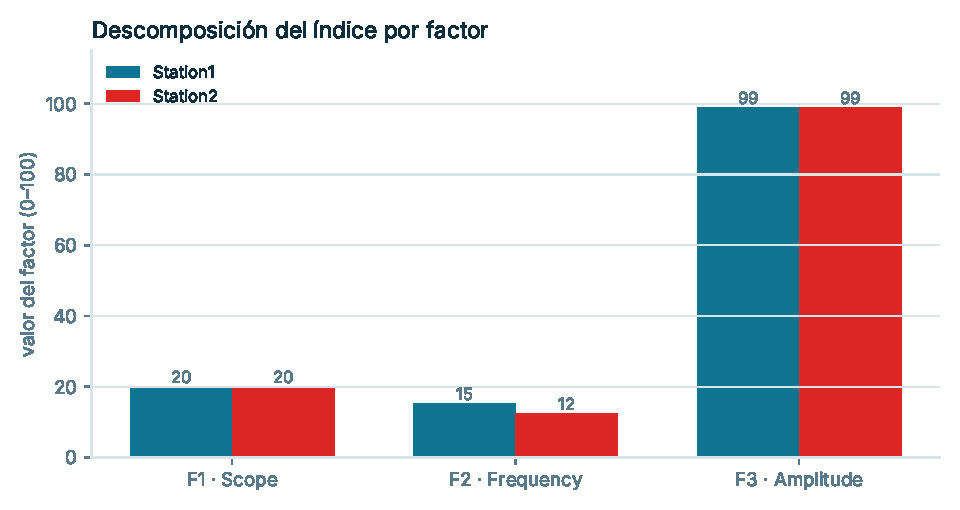
\includegraphics[width=0.7\textwidth]{manual_assets/factors.pdf}
\caption{Descomposición por factor en dos estaciones reales (agua ácida rica en aluminio): el resultado
``Mala'' está gobernado por $F_3$ (amplitud), no por la cantidad de parámetros que fallan.}
\end{figure}

\begin{okbox}[Verificación en la app]
ICA incluye este dataset como ``ejemplo del manual'' cargable con un clic. En producción reproduce
exactamente \textbf{WQI = 88}, categoría ``Buena'', con la narrativa: \emph{2 de 10 parámetros
incumplieron su guía (PB, TP), en 4 de 103 pruebas} —idéntico al manual—.
\end{okbox}

% =================== PARTE IV ===================
\part{El sitio ica.endho.mx}

\section{Cómo usar ICA: los cuatro pasos}
La app organiza el trabajo en un asistente de cuatro pasos, con navegación por pestañas.

\subsection{\texorpdfstring{Paso \ding{192} Guías}{Paso 1 Guias}}
Elige un punto de partida: un \textbf{preset} (CCME o la plantilla México), \textbf{sube tu propio}
\texttt{Guidelines} (CSV/Excel) o \textbf{empieza de cero}. Luego edita la tabla, agrega parámetros con
el asistente (catálogo de DBO, DQO, fluoruro, E.\,coli\dots) y observa la validación en vivo.

\shot{manual_assets/site_guias.png}{0.92\textwidth}

\subsection{\texorpdfstring{Paso \ding{193} Datos}{Paso 2 Datos}}
Sube tu monitoreo en \textbf{formato ancho} (columnas \texttt{Station}, \texttt{Date}, y una columna por
parámetro), en CSV o Excel. ICA valida de forma cruzada: emparejamiento de columnas contra la guía,
dependencias (dureza/pH/temperatura), tipos y rangos, y habilita una compuerta \textbf{``Listo para
calcular''} cuando no hay errores.

\subsection{\texorpdfstring{Paso \ding{194} Resultados}{Paso 3 Resultados}}
Por cada estación: un \textbf{medidor} 0–100 con la categoría, una \textbf{narrativa} en español, la
\textbf{descomposición F1/F2/F3}, la \textbf{tendencia por año} y un \textbf{mapa de calor de
excedencias} (parámetro × fecha, coloreado por magnitud). Todo exportable a CSV.

\shot{manual_assets/site_resultados.png}{0.82\textwidth}

\subsection{\texorpdfstring{Paso \ding{195} Ayuda}{Paso 4 Ayuda}}
Un tutorial con el ejemplo del manual cargable con un clic (para comprobar el WQI=88), más la
explicación del índice, las ecuaciones, las categorías y buenas prácticas.

\section{Formato de datos y de guías}
\begin{keybox}[Formato ancho de datos]
Primera columna \texttt{Station}, segunda \texttt{Date} (acepta \texttt{M/D/AAAA}, \texttt{D-Mon-AA} o
\texttt{AAAA-MM-DD}), y después una columna por parámetro. Los valores bajo el límite de detección se
escriben como \texttt{<0.01}. Las celdas vacías son datos faltantes.
\end{keybox}
El nombre de cada columna de datos debe coincidir \textbf{exactamente} con el \texttt{PARAMETER\_ID} de
la guía; ICA reporta las columnas sin guía y las guías sin datos.

\section{Autoguardado, proyecto y privacidad}
\begin{sitebox}[Tu trabajo, tuyo]
ICA \textbf{autoguarda} el proyecto en tu navegador (sobrevive a recargas) y permite \textbf{exportar/
importar} un archivo \texttt{.ica.json} con la guía y los datos, para respaldar o compartir. No hay
cuentas ni servidor: \textbf{ningún dato sale de tu equipo}.
\end{sitebox}

% =================== PARTE V ===================
\part{Criterio, estado y referencias}

\section{Ventajas y limitaciones}
\begin{minipage}[t]{0.49\textwidth}
\textbf{Ventajas}
\begin{itemize}[leftmargin=1.1em,nosep]
  \item Comunica datos complejos en un número.
  \item Sin ponderaciones arbitrarias.
  \item Escala-invariante (mezcla µg/L, mg/L, conteos).
  \item Robusto ante rangos extremos (asíntota de $F_3$).
  \item Trazable (tres factores interpretables).
\end{itemize}
\end{minipage}\hfill
\begin{minipage}[t]{0.49\textwidth}
\textbf{Limitaciones}
\begin{itemize}[leftmargin=1.1em,nosep]
  \item Pérdida de información (un solo número).
  \item Sensible a qué parámetros/guías se eligen.
  \item Fronteras de categoría subjetivas.
  \item Ciego a eventos transitorios.
  \item Falsos positivos por LD antiguos.
\end{itemize}
\end{minipage}

\section{La guía mexicana: estado provisional y ruta de validación}
\begin{warnbox}[Importante — leer antes de usar la plantilla México]
El \textbf{motor} de ICA está validado (reproduce el WQI=88 oficial). En cambio, la \textbf{plantilla
México} y el \textbf{catálogo del asistente} traen valores \textbf{PROVISIONALES}, marcados como tales,
que \textbf{deben verificarse} contra la norma vigente antes de usarse como definitivos:
NOM-127-SSA1-2021 (uso y consumo humano), CE-CCA-001/89 y NOM-001-SEMARNAT-2021 (criterios
ecológicos/descargas), y OMS.
\end{warnbox}
La siguiente etapa del proyecto es de \textbf{criterio científico}, no de código: decidir el uso
objetivo (potable / vida acuática / tipo CONAGUA), anclar cada valor de parámetro a su norma con la
fuente citada, y que un experto revise las fórmulas dependientes de dureza/pH. Hecho eso, la plantilla
mexicana pasaría de provisional a definitiva.

\section{Referencias}
\begin{itemize}[leftmargin=1.4em,label={}]
\item CCME. 2017. \emph{Canadian Water Quality Guidelines for the Protection of Aquatic Life: CCME Water Quality Index, User's Manual — 2017 Update.} Winnipeg.
\item CCME. 2001. \emph{CCME Water Quality Index 1.0, Technical Report.}
\item Rocchini, R. y L.G. Swain. 1995. \emph{The British Columbia Water Quality Index.}
\item Wright, C.R. et al. 1999. \emph{A Water Quality Index for Agricultural Streams in Alberta (AAWQI).}
\item Fichas CCME por sustancia: Cadmio \url{https://ccme.ca/en/chemical/20}; Cobre \url{https://ccme.ca/en/chemical/71}; Níquel \url{https://ccme.ca/en/chemical/139}.
\item Normas mexicanas de referencia: NOM-127-SSA1-2021; CE-CCA-001/89; NOM-001-SEMARNAT-2021; guías OMS.
\end{itemize}

\vfill
\begin{center}\small\color{muted}
\rule{0.4\textwidth}{0.4pt}\\[4pt]
Guía de referencia de \textbf{ICA} · \href{https://ica.endho.mx}{ica.endho.mx}. Las ecuaciones y valores
de guía son hechos técnicos publicados por el CCME; las explicaciones, figuras, capturas y el análisis
son elaboración propia. \today
\end{center}

\end{document}
